\chapter{Desired Solution}
\section{User Story Video}
Based on the functional requirements, and after receiving inspiration form evaluating existing solutions, the team came up with a design suggestion together with the customer. To present the vision we had of what a solution could look like, the team created a user story video \cite{video} in which several scenarios of interacting with the solution where presented. The video also explained how the different users came into contact with the solution and why they begun using it. The story line of the video can be seen here, Figure \ref{fig:video}, with images from the video depicting the most important use cases of the solution. 

\begin{figure}[H]
\centering
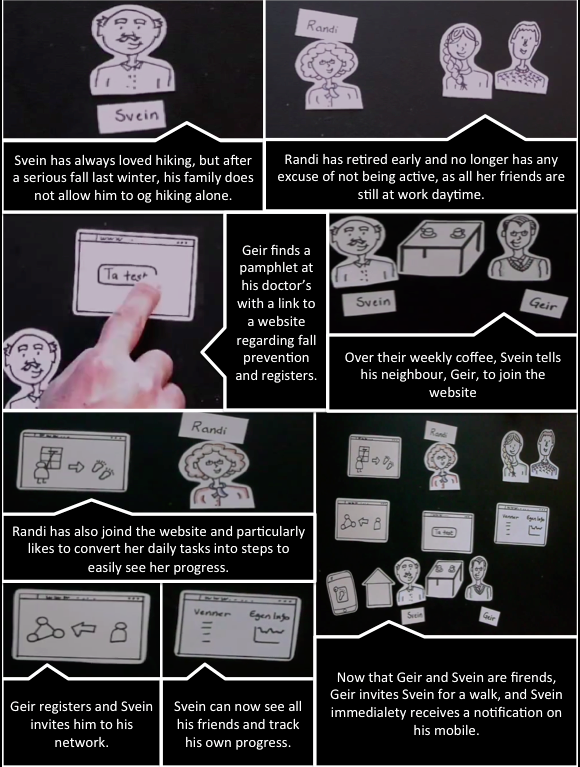
\includegraphics[width = 0.75\textwidth]{Figures/VideoImages}
\caption{Story board of user story video}
    \label{fig:video}
    \end{figure}

\section{Wireframes}
Moving on from the concept displayed in the video, the team made wireframes and mock-ups to display the initial ideas of what the solution could look like. This is how we initially envisioned the system: 


\begin{figure}[H]
\centering
 \textbf{Web-based Solution}\par\medskip
\begin{subfigure}{.5\textwidth}
  \centering
  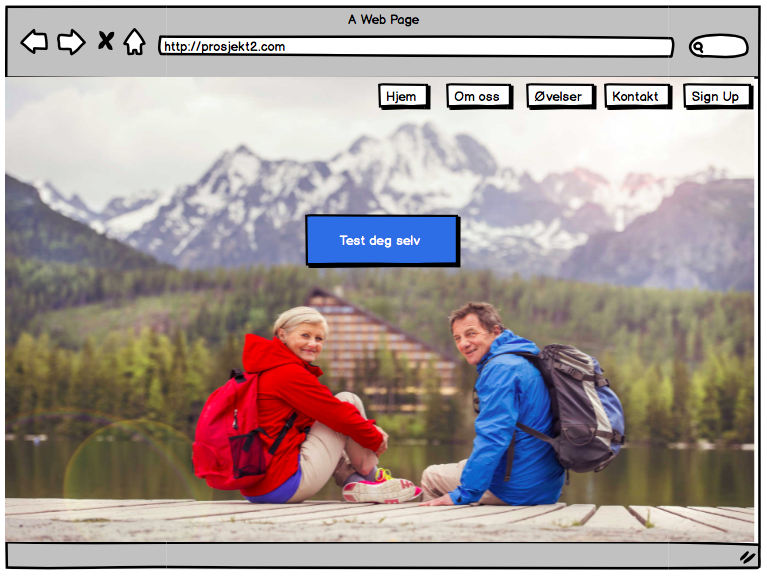
\includegraphics[width=.8\linewidth]{wireframes/web/Home}
  \caption{Home page of web application, where the test is the focal point.}
  \label{fig:videoHome}
\end{subfigure}%
\begin{subfigure}{.5\textwidth}
  \centering
  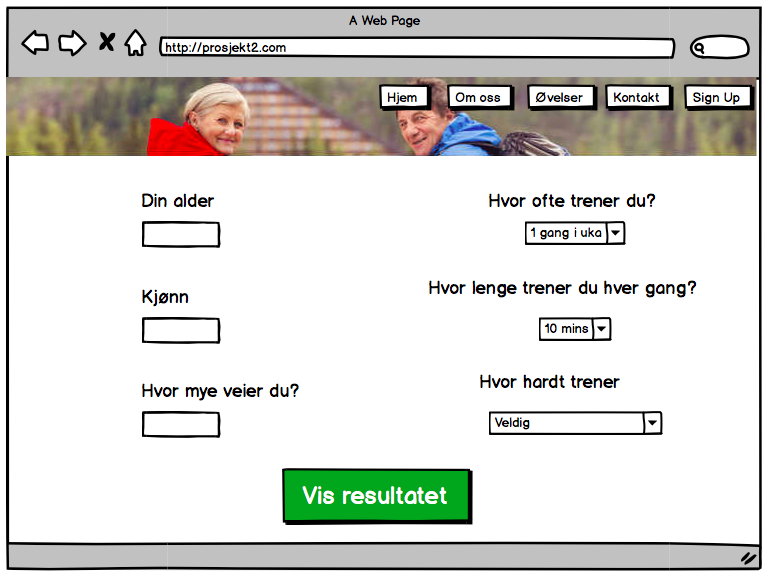
\includegraphics[width=.8\linewidth]{wireframes/web/TestDetails}
  \caption{Test interface}
  \label{fig:videoTest}
\end{subfigure}\\
\break
\begin{subfigure}{.5\textwidth}
  \centering
  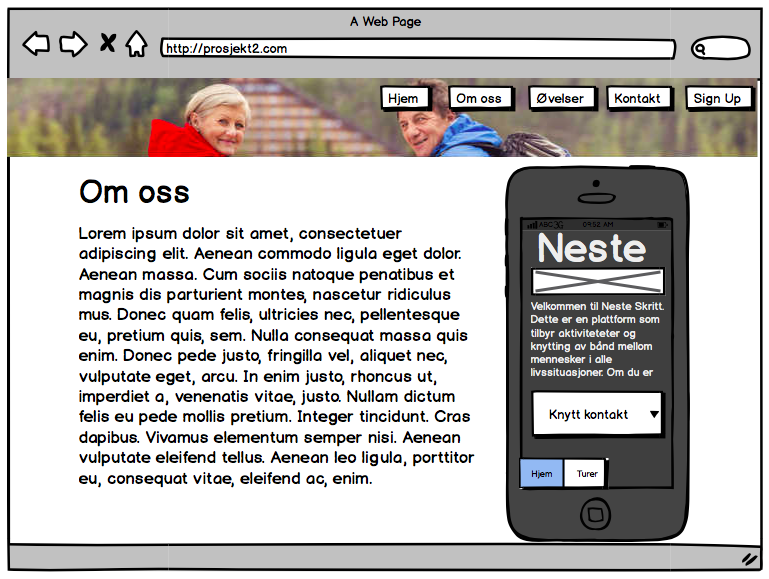
\includegraphics[width=.8\linewidth]{wireframes/web/About}
  \caption{About Us page. If the name was changed to info, this page could also serve as the source of information about fall risk and prevention.}
  \label{fig:videoAbout}
\end{subfigure}%
\begin{subfigure}{.5\textwidth}
  \centering
  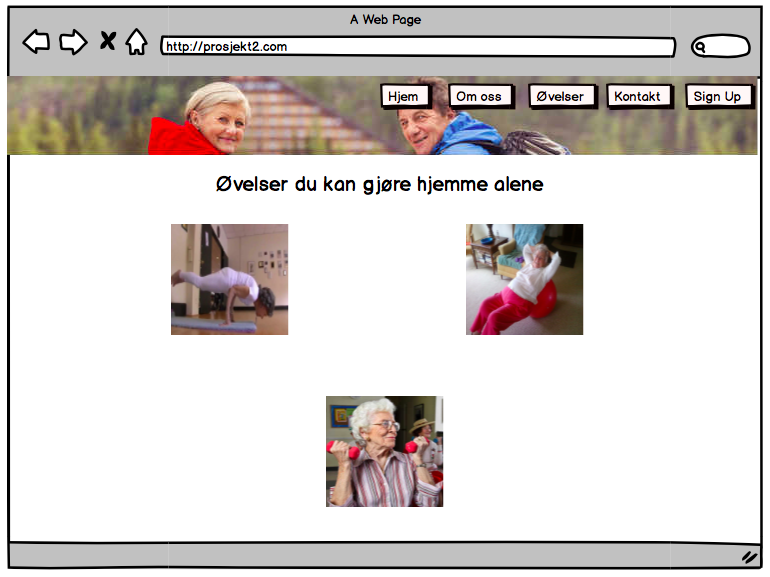
\includegraphics[width=.8\linewidth]{wireframes/web/Activities}
  \caption{Activities page: the different activities are displayed here.}
  \label{fig:videoACtivities}
\end{subfigure}\\
\break
\begin{subfigure}{.5\textwidth}
  \centering
  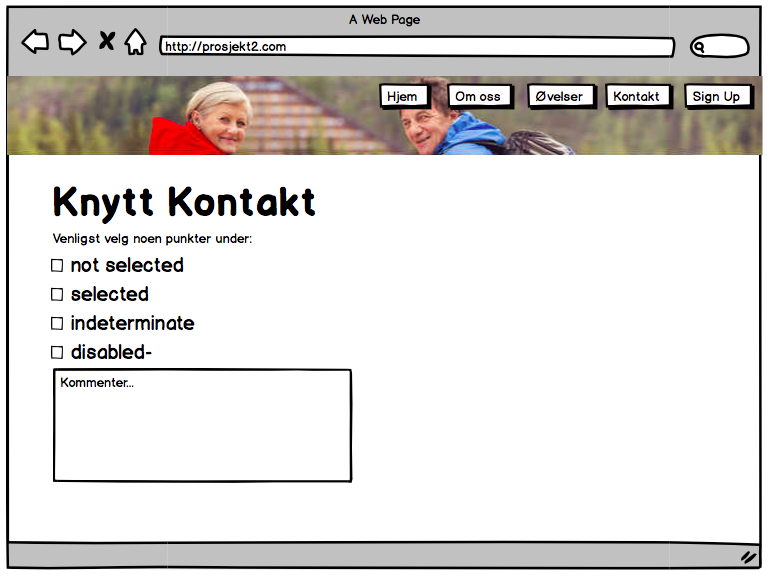
\includegraphics[width=.8\linewidth]{wireframes/web/Contact}
  \caption{Contact: a page where one can make acquaintances without necessarily registering to the service. }
  \label{fig:videoContact}
\end{subfigure}%
\begin{subfigure}{.5\textwidth}
  \centering
  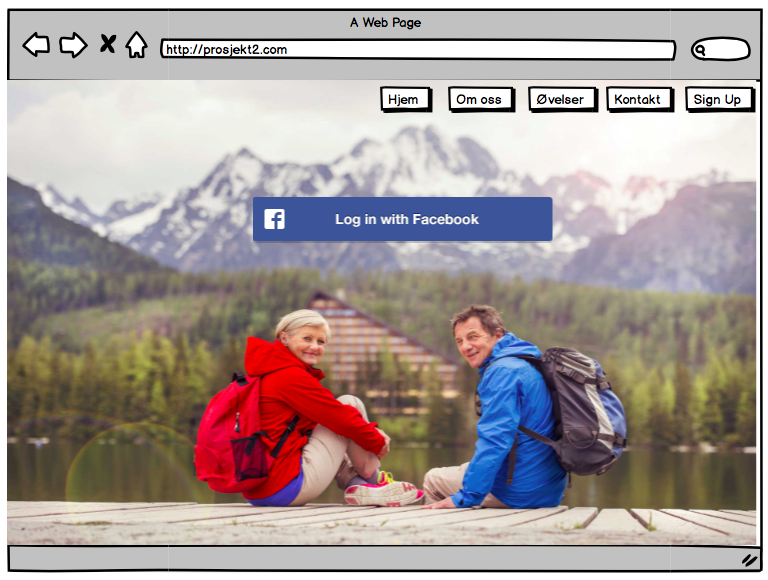
\includegraphics[width=.8\linewidth]{wireframes/web/SignUp}
  \caption{SignUp page: here users can sign in with Facebook to avoid long registration forms. The final solution could possibly include google-signIn as well, and perhaps a custom registration for  for users with none of the above-mentioned accounts.}
  \label{fig:videoSignUp}
\end{subfigure}
\caption{Wireframes for web solution}
\end{figure}

    

\begin{figure}[H]
\centering
 \textbf{Mobile Application}\par\medskip
\begin{subfigure}{.5\textwidth}
  \centering
  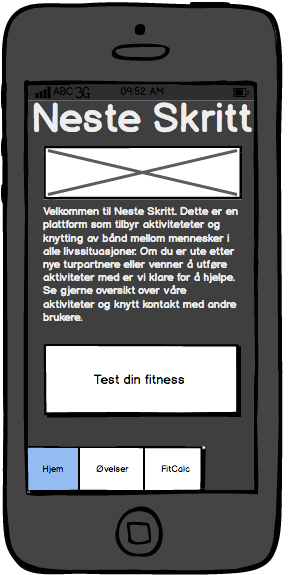
\includegraphics[width=.5\linewidth]{wireframes/app/Home}
  \caption{Home page}
  \label{fig:appHome}
\end{subfigure}%
\begin{subfigure}{.5\textwidth}
  \centering
  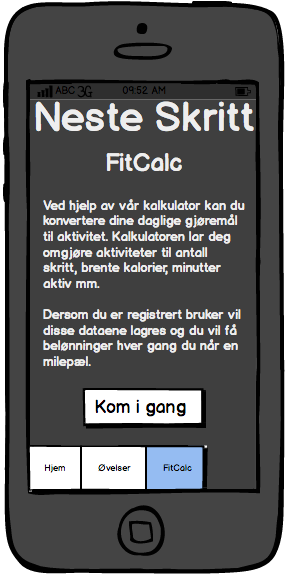
\includegraphics[width=.5\linewidth]{wireframes/app/Test}
  \caption{Test page}
  \label{fig:appTest}
\end{subfigure}\\
\begin{subfigure}{.5\textwidth}
  \centering
  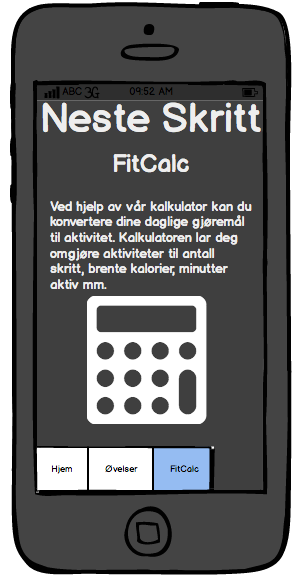
\includegraphics[width=.5\linewidth]{wireframes/app/Calc}
  \caption{Activity converter}
  \label{fig:appCalc}
\end{subfigure}\\
\begin{subfigure}{.5\textwidth}
  \centering
  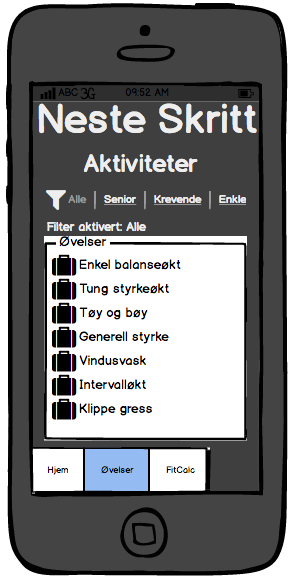
\includegraphics[width=.5\linewidth]{wireframes/app/Activities}
  \caption{Activities page}
  \label{fig:appActivities}
\end{subfigure}%
\begin{subfigure}{.5\textwidth}
  \centering
  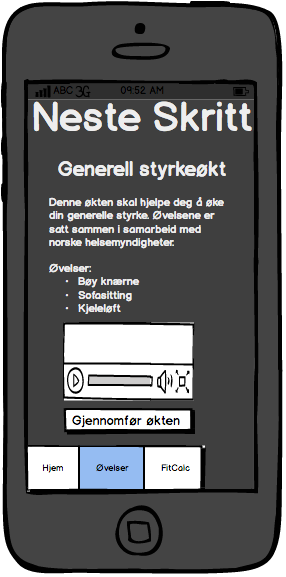
\includegraphics[width=.5\linewidth]{wireframes/app/Activity}
  \caption{Page for displaying an individual activity}
  \label{fig:appActivity}
\end{subfigure}
\caption{Wireframes for mobile application}
\end{figure} 


